% DO NOT COMPILE THIS FILE DIRECTLY!
% This is included by the other .tex files.

\begin{frame}[t,plain]
    \titlepage
\end{frame}

\begin{frame}
    \frametitle{Objectives of this module}
    \begin{itemize}
        \item Tips for joining information sharing communities
        \item Tips for being a good member in a sharing community
        \item Tips for building your own sharing community
        \item Tool for managing a sharing community
        \begin{itemize}
            \item Managing organisations and contacts
            \item Maintaining distribution lists (aka sharing groups)
            \item Managing a large cluster of MISPs
        \end{itemize}
    \end{itemize}
\end{frame}

\section{Being part of an information sharing community}
\begin{frame}
    \frametitle{Joining an information sharing communities}
    There is a wide range of MISP communities type:
    \begin{itemize}
        \item Private sector communities
        \begin{itemize}
            \item Private organisations, researchers, central hub
        \end{itemize}
        \item ISACs communities
        \begin{itemize}
            \item Central hub for sectorial or geographical Communities
            \item Examples: GSMA, FIRST.org, CSIRT Network, Banking, etc
        \end{itemize}
        \item Ad-hoc communities
        \begin{itemize}
            \item Often use for exercises such as ENISA or LockedShield
        \end{itemize}
    \end{itemize}
\end{frame}

\begin{frame}
    \frametitle{Joining an information sharing communities}
    Considerations before joining a sharing community:
    \begin{itemize}
        \item Understand the community's objectives
        \begin{itemize}
            \item Defense, prevention, collaboration, research, specific reporting duties
        \end{itemize}
        \item Make sure the use-cases are not conflicting
        \begin{itemize}
            \item False-positive appetite, maturity levels, topical interests
            \item Detection rules VS threat intelligence VS prevention
        \end{itemize}
    \end{itemize}
\end{frame}

\begin{frame}
    \frametitle{Tips for being a good member of a sharing community}
    \begin{itemize}
        \item As explained extensively in course \textit{e.206}, Context is king:
        \begin{itemize}
            \item You should try to contextualise as best as you can using:
            \item Normalized vocab: Taxonomies, Galaxies \& MITRE ATT\&CK
            \item Connected graph using MISP Objects and relationships
            \item Add timeliness with Sightings and \texttt{first\_seen} / \texttt{last\_seen}
        \end{itemize}
        \item Sharing results and reports
        \item Sharing enhancements or proposals to existing data
        \item Validating data (sightings) or flagging false positives
        \item Asking for support from the community
    \end{itemize}
\end{frame}

\begin{frame}
    \frametitle{Tips for building your own sharing community}
    \begin{itemize}
        \item Different models for your constituents
        \begin{itemize}
            \item {\bf Having an account} on a MISP instance
            \item {\bf Hosting} their own instance and connecting to a peer
            \item {\bf Becoming member} of a sectorial MISP community that is connected to multiple peers
        \end{itemize}
        \item Planning ahead for future growth
        \begin{itemize}
            \item Estimating requirements (workforce, hardware requirements)
            \item Deciding early on common vocabularies (i.e. taxonomies)
            \item Offering services through MISP to promote adhesion
        \end{itemize}
    \end{itemize}
\end{frame}

\begin{frame}
    \frametitle{Tips for building your own sharing community}
    \begin{itemize}
        \item {\bf Lead by example} - the power of immitation
        \item Don't block sharing with unrealistic quality controls
        \begin{itemize}
            \item You might loose organisations that might turn into valuable contributors
            \item Organisations will start sharing junk to stay above the thresholds
        \end{itemize}
        \item Encourage {\bf improving by doing}
        \begin{itemize}
            \item What should the information look like?
            \item How should it be contextualised
            \item What do you consider as useful information?
            \item What tools did you use to get your conclusions?
        \end{itemize}
    \item Side effect is that you will end up {\bf raising the capabilities of your constituents}
    \end{itemize}
\end{frame}

\begin{frame}
    \frametitle{Tips for building your own sharing community}
    \begin{itemize}
        \item Convert the passive organisations into actively sharing ones
        \begin{itemize}
            \item Help them increase their capabilities
            \item Lead by example
            \item \textbf{Give credit where credit is due}
            \begin{itemize}
                \item Never steal the contribution of your community
            \end{itemize}
            \item Offers the possiblity to take over their data via \textbf{delegation}
            \begin{itemize}
                \item Anonymity of organisations might help them building confidence at the beginning
            \end{itemize}
        \end{itemize}
    \end{itemize}
\end{frame}

\begin{frame}
    \frametitle{Tips for building your own sharing community}
    \begin{itemize}
        \item Encourage sharing of supporting materials, scripts or guidance for protection
        \item Raise awareness about the benefits of a well modelled, graph-based information
        \item Again, \textbf{context is king}! If possible, make contextualisation a requirement
        \begin{itemize}
            \item Users can then filter based on their needs
            \item Classification help your peers to understand why the data is important
            \item And also, why this data can be useful to them
        \end{itemize}
    \end{itemize}
\end{frame}

\begin{frame}
    \frametitle{Dispelling the myths around blockers when it comes to information sharing}
    \begin{itemize}
        \item Sharing difficulties are not really technical issues but often it's a matter of {\bf social interactions} (e.g. {\bf trust}).
        \begin{itemize}
            \item You can play a role here: organise regular workshops, conferences, have face to face meetings
        \end{itemize}
        \item Legal restrictions
        \begin{itemize}
            \item "Our legal framework doesn't allow us to share information."
            \item "Risk of information leak is too high and it's too risky for our organization or partners."
        \end{itemize}
        \item Practical restrictions
        \begin{itemize}
            \item "We don't have information to share."
            \item "We don't have time to process or contribute indicators."
            \item "Our model of classification doesn't fit your model."
            \item "Tools for sharing information are tied to a specific format, we use a different one."
        \end{itemize}
    \end{itemize}
\end{frame}

\begin{frame}
    \frametitle{Managing sub-sharing communities}
    \begin{itemize}
        \item Often within a community, \textbf{smaller bubbles} of information sharing will form
        \begin{itemize}
            \item e.g: Within a national private sector community, a dedicated community for financial institutions
            \item If an incident involves multiple organisations
        \end{itemize}
        \item MISP's sharing group serve this purpose mainly
        \item If you are building your own community, consider bootstraping these specific sharing community
        \begin{itemize}
            \item Organisations can self-organise, but you are probably the ones with the know-how to get them started
        \end{itemize}
    \end{itemize}
\end{frame}

\section{Community management and orchestration tool}
\begin{frame}
    \frametitle{Additional challenges of community management}
    \begin{itemize}
        \item MISP is just one part of the puzzle
        \item Information sharing presumes knowledge of contacts
        \item Creating reusable community-specific distribution list need to be maintained
        \item Fleet management for larger organisations needs additional work
    \end{itemize}
    \begin{center}
        \textbf{Cerebrate} is an open-source tool meant to address these challenges
    \end{center}
\end{frame}

\begin{frame}
    \frametitle{What is Cerebrate?}
    \begin{center}
        
\includegraphics[scale=0.10]{pictures/cerebrate-logo.png}
    \end{center}
    \begin{itemize}
        \item Open source {\bf community management and orchestration} tool
        \item Central tool for the Melicertes 2 project (Co-funded by the EU as a CEF project)
        \begin{itemize}
            \item Project for the CSIRT network building a common set of tools and services for the national CSIRTs
            \item Flexible to support a wide range of communities
        \end{itemize}
        \item Tight \textbf{integration} with various open-source tools
        \item Planned as the primary MISP management tool
    \end{itemize}
\end{frame}

\begin{frame}
    \frametitle{Why do we need Cerebrate from a MISP perspective}
    \begin{itemize}
        \item {\bf Deficiencies} in our current tool chain
        \begin{itemize}
            \item Do I really have to jump through hoops and long e-mail chains to {\bf onboard new members}?
            \item How do I {\bf find trusted information} on who an organisation is in MISP?
            \item How can I {\bf manage a large cluster of MISPs} without tedious manual labour?
            \item If I run a community through MISP, how can I reuse my member information for other community tasks such as mailing lists?
            \item Information signing has been on the MISP roadmap for a long time - where do we get ground truths for a community from?
        \end{itemize}
    \end{itemize}
\end{frame}

\begin{frame}
    \frametitle{What issues is Cerebrate trying to tackle?}
    \begin{itemize}
        \item Community management
        \begin{itemize}
            \item {\bf Repository} of organisations and individuals
            \item Management of {\bf sharing groups}
            \item {\bf Exchange} of contact and sharing group information
            \item Cryptographic key lookup for {\bf information signing}
        \end{itemize}
        \item Local tool management
        \begin{itemize}
            \item Instrumentation of {\bf local tool interconnections}
            \item Local tool {\bf fleet management}
            \item {\bf Feeding} the local tools with Cerebrate data
        \end{itemize}
    \end{itemize}
\end{frame}

\begin{frame}
    \frametitle{Cerebrate: What is available currently?}
    \begin{itemize}
        \item A set of Common functionalities
        \item Contact Database
        \item Sharing group management
        \item Cerebrate to Cerebrate synchronisation
        \item Mailing list management
        \item Local tool orchestration - integration modules
        \item Inbox system
        \item Local tool fleet management
    \end{itemize}
\end{frame}

\begin{frame}
    \frametitle{Cerebrate: Contact database}
    \begin{itemize}
        \item Index of Organisations and Individuals
        \item Flexible meta-data model (community specific, constituency, etc)
        \item Content aware search functionalities
    \end{itemize}
\end{frame}

\begin{frame}
    \frametitle{Cerebrate: Contact database}
    Flexible meta-data model to include community specific data point
    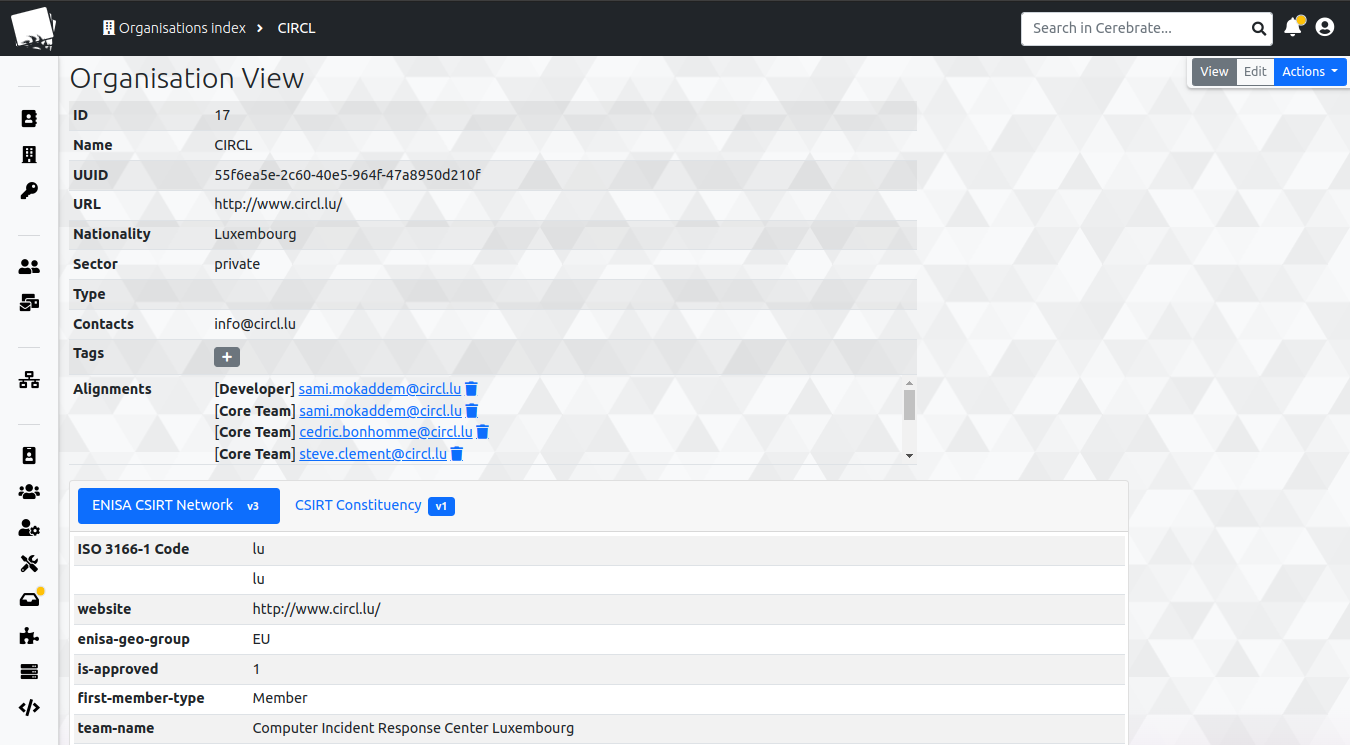
\includegraphics[width=0.99\linewidth]{pictures/cerebrate1.png}
    \note[item]{Cerebrate includes a system to support meta-data that can be attached to existing enties}
    \note[item]{This system is composed of meta-template which defines additional data-point}
    \note[item]{It can be used to create new structure unknown to a default Cerebrate installation}
\end{frame}

\begin{frame}
    \frametitle{Cerebrate: Contact database}
    Content aware search functionalities: CIDR block search
    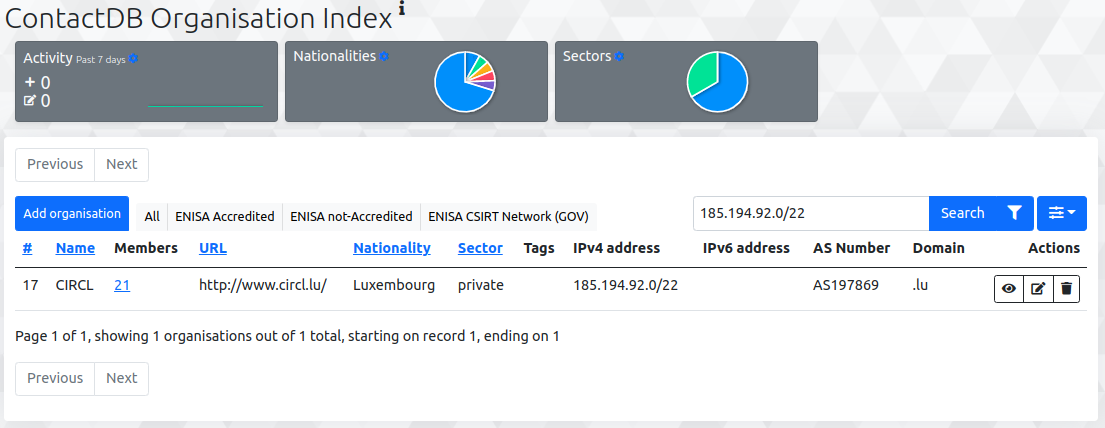
\includegraphics[width=0.99\linewidth]{pictures/cerebrate2.png}
    \note[item]{The meta-template system also support different data type}
    \note[item]{In this screenshot, we can a search for an IP address and the matching CIDR block is returned}
\end{frame}

\begin{frame}
    \frametitle{Cerebrate: Contact database}
    Global searches on a large variety of data point
    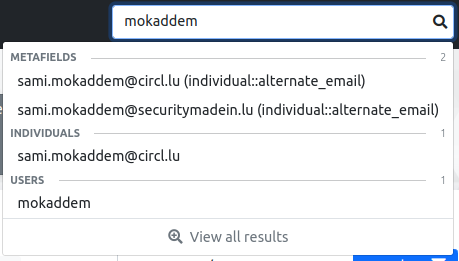
\includegraphics[width=0.99\linewidth]{pictures/cerebrate3.png}
    \note[item]{The tool allows users to search in a multiple of scope at the same time}
\end{frame}

\begin{frame}
    \frametitle{Cerebrate: Sharing Group management}
    Allow to define sharing groups composed of organisations that can be download from another Cerebrate or from MISP
    \begin{center}
        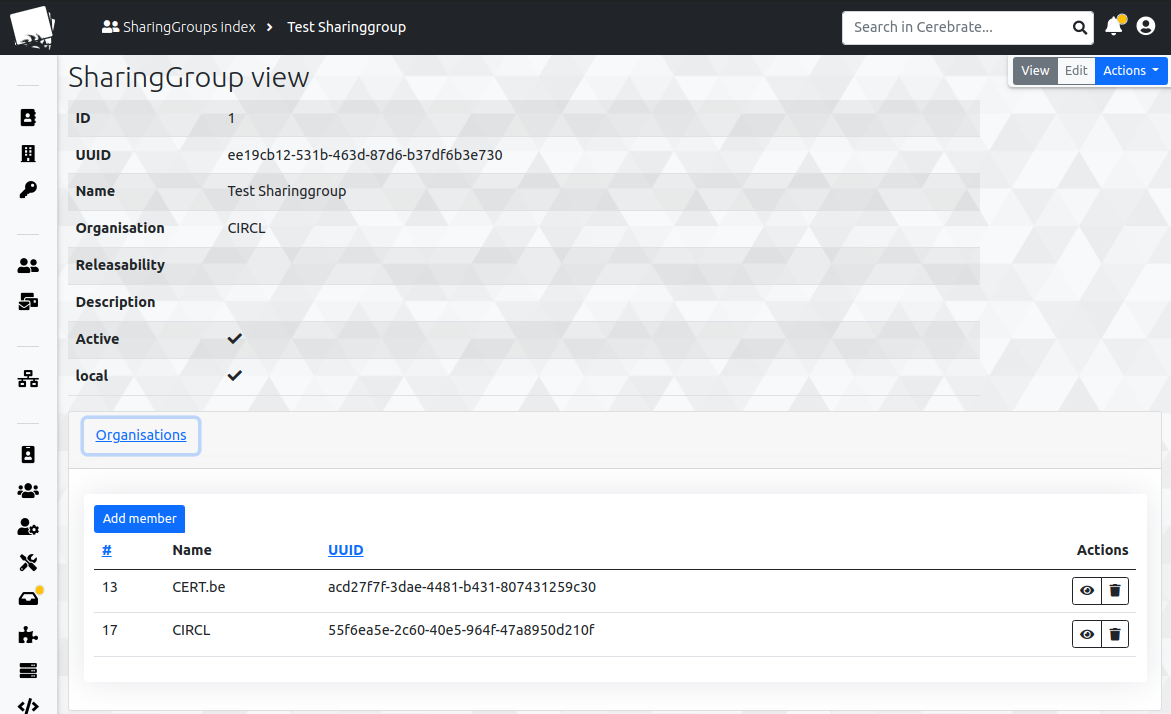
\includegraphics[width=1.00\linewidth]{pictures/cerebrate-sg.png}
    \end{center}
    \note[item]{In this screenshot, we can see a sharing group composed of two organisations: CIRCL and cert.be}
\end{frame}

\begin{frame}
    \frametitle{Cerebrate: Sharing Group management}
    Sharing groups can also be generated based on filters via the reusable blueprints
    \begin{center}
        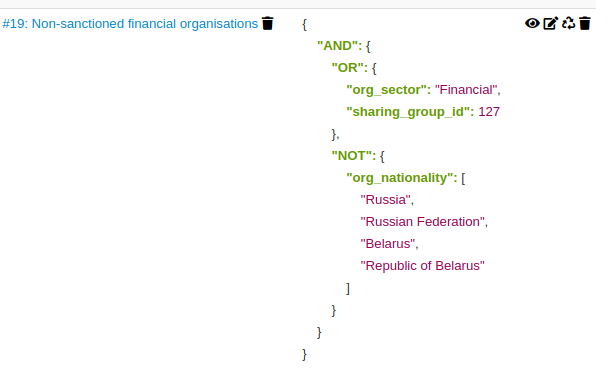
\includegraphics[width=0.88\linewidth]{pictures/misp-sg-blueprint.png}
    \end{center}
    \note[item]{In this screenshot, we can see a sharing group blueprint definition where}
    \note[item]{Organisation of the RU nationality are exluded}
    \note[item]{Organisation from the "Financial" sector are included}
    \note[item]{All organisation contained in the sharing group 127 are included}
\end{frame}

\begin{frame}
    \frametitle{Cerebrate: cerebrate-cerebrate synchronisation}
    Mechanism to exchange contact data via synchronisation
    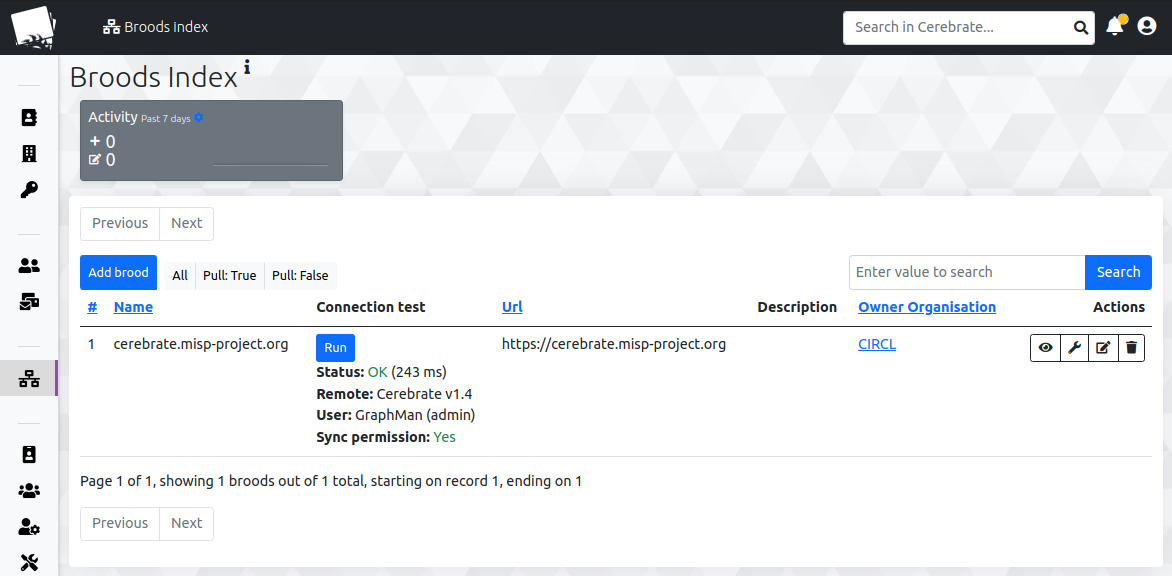
\includegraphics[width=1.0\linewidth]{pictures/cerebrate-brood.png}
    \note[item]{Similar to MISP, cerebrate suport data exchange to and from other Cerebrate instances}
\end{frame}

\begin{frame}
    \frametitle{Cerebrate: Local tool orchestration}
    Manage and configure local tools (such as MISP) via Cerebrate
    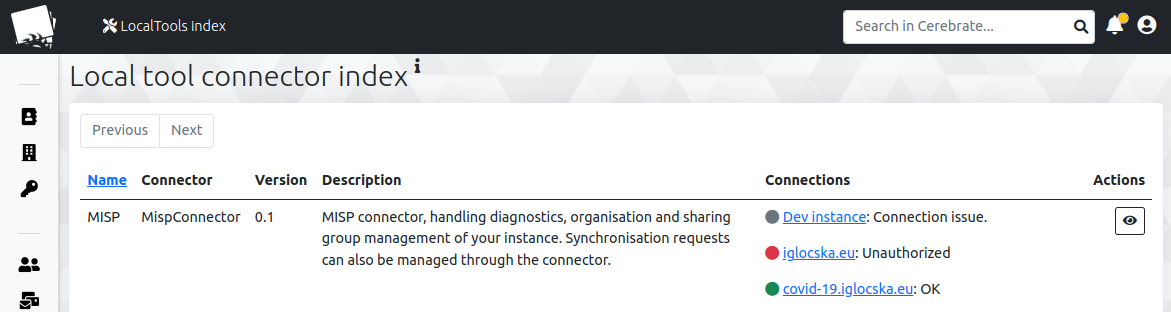
\includegraphics[width=1.0\linewidth]{pictures/cerebrate-lt.png}
    \note[item]{The screenshot shows that Cerebrate has a MISP connector}
    \note[item]{This connector is used to control 3 MISP instances where we can see their connection status}
\end{frame}

\begin{frame}
    \frametitle{Cerebrate: Local tool orchestration}
    Inter-connect local tools (such as a MISP instance) to another through Cerebrate
    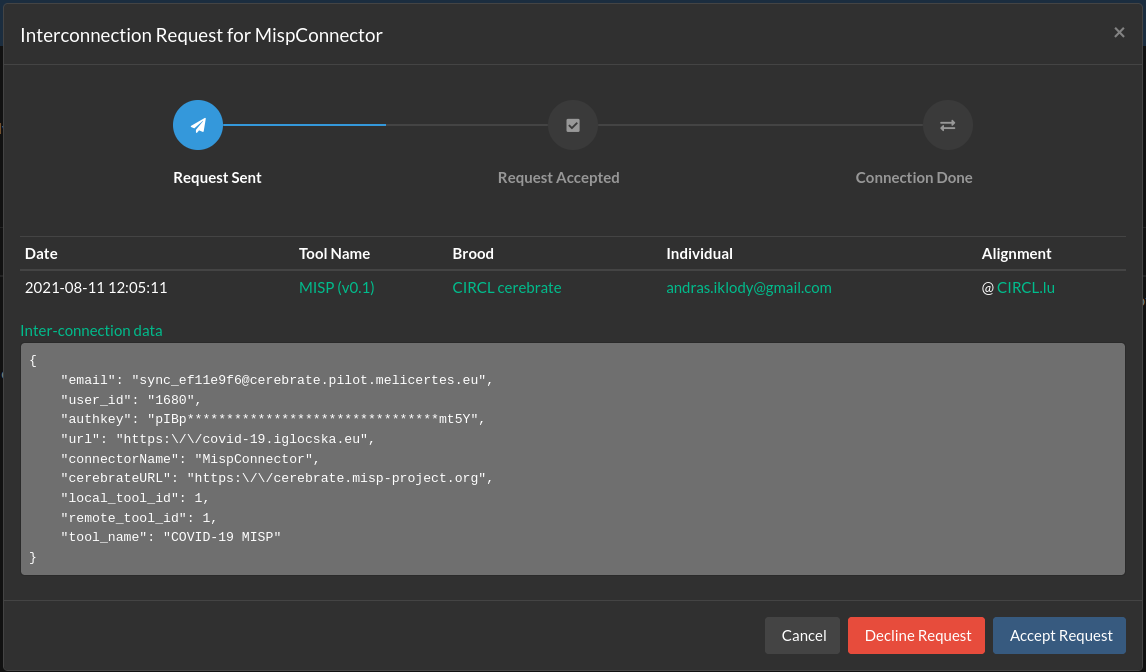
\includegraphics[width=1.0\linewidth]{pictures/cerebrate-inbox.png}
    \note[item]{The screenshot shows a message received from another Cerebrate instance}
    \note[item]{This message request the inter-connection of the local MISP instance with the MISP instance of the remote Cerebrate}
    \note[item]{To have the connection between the two MISP finalized, the user must accept the request, then the initiator must finalize it}
\end{frame}

\begin{frame}
    \frametitle{Use case specific to law enforcement}
    \begin{itemize}
        \item Budapest convention allowed us to have a public inventory of contact infomartion
        \item Once this data is ingested in Cerebrate, we can make use of the search functionalities to quickly get the infomartion we need
    \end{itemize}
    TODO: Include picture of data stored in Cerebrate
\end{frame}
